\documentclass[12pt]{article}

\title{Research paper}
\author{Wessel Stoop, s0808709}

\usepackage{covington}
\usepackage{graphicx}
\usepackage{natbib}

\renewcommand{\familydefault}{\sfdefault}

\begin{document}
\maketitle

\section{Introduction}

When one of Starfleet's vessels meets an alien ship in areas where no man has gone before, they can (almost) always communicate with these aliens (almost) instantly; they speak to them in English, and these aliens answer in English. This is possible because, according to the Star Trek lore, the protagonists make use of a so-called Universal Translator. This Universal Translator can (1) recognize speech in every language, (2) translate what it has 'heard' to any other language, (3) make its results audible with speech synthesis and (4) learn itself new languages when needed. Unfortunately, like many technologies in Star Trek, this is far from reality: there is lots of active research at the first three tasks in particular, but no software currently in existence can do this as perfect as the Universal Translator. \\\indent
In this paper, I will give a detailed overview of the research project Colibri, which basically is an attempt to improve the technology needed for the second task: automatically translating text from one language to another. More specifically, the project investigates the identification and extraction of constructions in natural language, and how these can be used in Machine Translation. These constructions can be of various lengths, and, importantly, can also contain one or more gaps. The constructions are not identified on the basis of explicit 'human' knowledge about language and grammar ('linguistic theory'), but are distilled from large amounts of text ('text corpora') with the help of context-sensitive machine-learning techniques. The Colibri project is carried out by Maarten van Gompel and supervised by Antal van den Bosch.
\\\indent
In section 2, I'll give a short overview of what has been achieved in machine translation, and in section 3 the current project will be described. This order was chosen to show that Colibri builds on previous research directly.

%Rest van de beschrijving.







\section{Theoretical background / framework}

In this section I will try to give a short overview of the various approaches in machine translation, with special attention to the example-based approach, as that is the approach used in this project. This section is mainly based on %Maartens thesis.

\subsection{The rule-based approach}

The rule-based approach, also known as Classical Machine Translation, is best characterized by the use of human created rules. That is, authors of translation algorithms tried to include their knowledge about the languages and translation. The rule-based approache can be subdivided into four subapproaches, summarized in the Vauquois triangle: \\

\begin{figure}[htb]
\centering
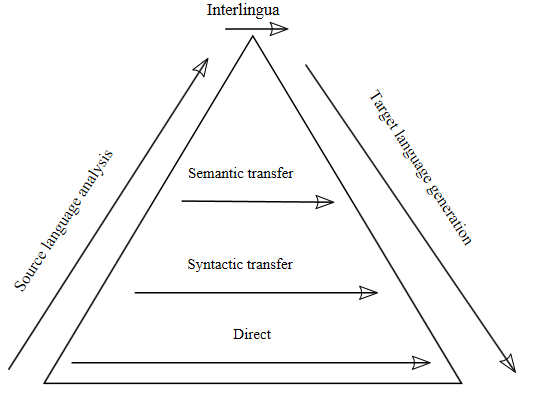
\includegraphics[width=0.8\textwidth]{vauquois.png}
\caption{The Vauquois triangle}
\label{fig:vauquois}
\end{figure}

The horizontal arrows represent the approaches. I'll go through them from bottom to top:

\begin{itemize}
\item \emph{The direct approach} does very little source language analysis, and could thus be viewed as the automatical version of looking up every word in the source language in a dictionary and replacing it with the corresponding word in the target language. This often doesn't yield very good results: if I for example would have translated this paper from my mother tongue Dutch to English word for word, 'would we now not real a good result have'. It should be noted, however, that the direct approach mostly is more complicated than this; for example, in some cases morphological analysis is needed before it can be looked up in a dictionary, and more morphological analysis is needed for the translation word to fit in the sentence. Word reordering rules can also be included.
\item \emph{The syntactic approach} tries to find out the syntactic structure of the source sentence before it starts translating, using a parser. This structure is then translated to the target language, and filled with translated words.
\item \emph{The semantic approach} goes even one step further and also tries to grasp the meaning of a sentence, roughly. For a sentence like /emph{Mummy kisses daddy} this for example entails that mummy is the agent, and daddy the patient of the sentence. After having identified these semantic roles, the algorithm would then look how this meaning is expressed in the target language, find the approriate syntactic structure for that, and fill it with the translated words.
\item \emph{The interlingua approach}. All of the approaches so far have in common that they require a seperate rule set for each language pair; no or very few rules included for translations from English to German can also be used for translations from English to French. The Interlingua approach is an attempt to solve this problem, by pairing up every language with a formal representation of meaning, the Interlingua. This means a translation from English to German would entail a translation from English to the Interlingua (using the ruleset English $\rightarrow$ Interlingua) and then a translation from the Interlingua to German (using the ruleset Interlingua $\rightarrow$ German). When translating from English to French, the same two steps would be taken, and the same ruleset English $\rightarrow$ Interlingua can be used. 
\end{itemize}

An advantage of the rule-based approach is that one has a lot of control over the output. In theory, if something has gone wrong, all one has to do is find out which rule or dictionary item caused the problem and improve it. In practice, however, it is almost impossible to have a dictionary and rule system good enough for more complicated sentences, and things like rule interactions and ambiguity make everything even more complicated. The next two approaches therefore replace hand-crafted rules with automatically generated ones.

% Voorbeelden? References?

\subsection{The statistical approach}

Unlike the ruled-based approach, the statistical approach creates its own 'knowledge', using bilingual text corpora. With this knowledge, the algorithm is able to generate various translation hypotheses, from which the best one is chosen with various statistical measures. I will explain these stages in more detail:

\begin{itemize}
\item \emph{Corpus alignment.} Only having a bilingual corpus is not enough: for such corpus to be useful one also needs to know which parts of the sentence in language A correspond to which part of the sentence B. This is not only complicated by different word orders, but also by concepts that in language A take more or less words than in language B. A well-known word alignment algorithm is the Expectation Maximisation algorithm \citep{dempster77}. 

%GIZA++?

\item \emph{Hypothesis generation.} We now have some sort of automatically generated dictionary: for each word in language A, we know which words in language B are often used for it. On the basis of this knowledge, we can generate various possible translations. 

\item \emph{Hypothesis evaluation.} Which one of these possible translation is the best one is determined on the basis of two measures: faithfulness and fluency (which can also be called grammaticality). These measures often are in conflict: a solution to get an optimally fluent translation would be to always return the same well-formed sentence, but that would not be faithful to the source language at all, while a very faithful translation, for example translating a sentence word by word, is usually not considered very fluent. Faithfulness and fluency are measured by the translation model and the language model respectively:

\begin{itemize}
\item \emph{The translation model.} The translation model returns a probability of source sentence given the target sentence; it thus looks back whether what has been created fits the original. This probability is calculated on the basis of statistical word alignment algorithms like the IBM models \citep{brown93}.

\item \emph{The language model.} The language model predicts to what extent the generated sentence is expected for the target language; in other words, is this sentence a well-formed sentence or not? Because the unlimited number of ways words can be combined into sentences, it is unlikely the sentence under investigation will actually be found in a corpus, so the language model tries to do this prediction on the basis of how often smaller parts of the sentence (n-grams) occur in a corpus.

\end{itemize}

\end{itemize}

\subsection{The example-based approach}

In this section, I'll give an overview of the example-based approach. I'll focus on the memory-based version of the example-based approach in particular, because that is the version the Colibri project uses. Other versions of example-based machine translation might vary slightly. \\\indent
The memory-based approach is in many ways similar to the statistical approach - it too generates translations on the basis of large bilingual corpora, for instance. The main difference, however, is that it is context-sensitive; the idea is that the system will find another translation for \emph{left} in the sentence \emph{The toilets are at your left hand} than \emph{left} in the sentence \emph{Elvis has left the building}. \\\indent
In the memory-based approach, this context-sensitivy is achieved with the help of machine learning: by showing a so-called classifier lots of examples of something, and telling it in which class it belongs, it is able to predict the class of new examples. For example, we can give a classifier the external characteristics of 10.000 humans (for example length, type of cloths, length of hair), and also tell it whether these humans are male or female. If we then ask for the sex of a relatively short human, wearing a dress, with long hair, it will probably be able to tell us this is a woman. While this example only has two classes, it is in principle possible to use an unlimited number of classes. This is exactly what the memory-based approach does: on the basis of a particular word and its context (for example, its direct neighbours), a classifier in machine translation returns as a class the most likely n-gram. Thus, instead of human characteristics the classifiers are trained on words and their context from the source language, and instead of sex it uses n-grams from the target language as classes. \\\indent
There are two types of classifaction methods: \emph{eager learning} and \emph{lazy learning}. Whereas eager learning algorithms try to creating a small, abstract, general model, filtering out infrequent cases, lazy learning algorithms take into account everything they encounter. According to \citet{dvdb05}, for natural language processing the lazy learning approach works best, because infrequent cases are an important part of the knowledge needed. \\\indent
Like I did with statistical machine translation, I will now give an overview of the memory-based machine translation process, based on \citet{vdbb09}. For this example, I will describe a translator that uses trigrams, but it should be noted that the Colibri system uses n-grams of various lengths.

\begin{itemize}
\item \emph{Local phase.} In the description of \citet{vdbb09}, the local phase entails both training the classifier and actual classification, but I think it is important to make a sharp distinction here: whereas the training is done only once and \emph{before} actual translation, and could therefore be seen as 'preparing' the translation software for its task, the classification is done every time the user asks for a translation. Training consists of (1) aligning the bilingual corpus, using the word alignment algorithms described in the previous sections, (2) decomposing the corpus into trigrams, and (3) giving the results to the classifier as training material. The trigrams of the source language constitute the examples, the trigrams of the target language are the classes. Classification means (1) decomposing the source text into trigrams and (2) classifying each trigram. We end up with a list of trigrams in the target language.

\item \emph{Global phase.} In the global phase we try to merge the trigrams into one text. The part of the translation software responsible for this is called the \emph{decoder}. There might be a lot of overlap in the resulting trigram (for example: '\emph{\_ I love}', '\emph{I love you}' and '\emph{love you \_}'), making the decoder's task relatively easy. Such overlap might even give hints for the word order of the target language. In many cases, unfortunately, such overlap does not exist or is even misleading. As with statistical translation, here too we can pick the best translation hypothesis by using a language model and a translation model. 

% Constraint Satisfaction Inference

\end{itemize}

%Moet ik hier iets zeggen over phrase based?







\section{Project description}

Besides an attempt to discover more about the possibilities for machine translation technology, Colibri is also an attempt to actually develop this technology. The following project overview therefore necessarily also is an overview of the software.

\subsection{Pattern extraction}

Colibri, 'Constructions as Linguistics Bridges', investigates constructions (or patterns), as its name suggests. A construction can be any group of consecutive words (a so-called 'n-gram') in any natural language that in some way forms an entity. An example is 'on the basis of' in the following sentence:

\begin{examples}
\item On the basis of these ideas, software can be developed.
\end{examples}

Importantly, constructions can also have one or more gaps (so-called 'skip-grams'). 'from \_\_ point of view' in the following example, is a construction with one such gap. 

\begin{examples}
\item I understand things better when I look at them from his point of view.
\end{examples}

The gap is filled here is filled with 'his', but the construction 'from \_\_ point of view' can also be filled with many other words ('my', 'the', 'another', 'Obama's', etc.). This shows the advantage of skip-grams over n-grams for machine translation: whereas n-grams would only have been able to capture the construction 'point of view', because the word directly before 'point of view' is variable, skip-grams are also able to recognize that the word 'for' is part of the construction.\\\indent
Of course, not every possible group of consecutive words is a construction; what makes some groups special? The exact nature of linguistic constructions has been the subject of many publications and even an entire linguistic framework (construction grammar). For this project however, it suffices to say that constructions emerge because some combinations of words are more frequent than others.

% Drie vormen freq: raw frequency, context frequency, multilingual alignmetn
% Blabla, want freq is waar mach learning gebriuk van maakt

\subsection{Pattern querying} Interactively query generated models for specific patterns.
\subsection{Pattern/corpus comparison} Match patterns generated from one corpus to another corpus.
\subsection{Graph computation \& visualisation} Compute graph relations between pattern models and visualise graphs
\subsection{Alignment algorithms} Algorithms to extract and align patterns accross languages; resulting in translation pairs for constructions.
\subsection{Machine Translation Decoding} Reassembles translated fragments into one coherent sentence in the target-language; seeking the best (statistically most probably) solution in a vast search space of possible search hypotheses.
\subsection{Memory-based Machine Translation} Machine learning algorithms can be used to consider source-side context in translations. Classifiers can be built and directly used by the decoder.
\subsection{Experiment Framework} Colibri comes with an extensive experiment framework for conducting Machine Translation experiments.\

\subsection{Hypotheses} %Of moet dit bij main outstanding questions?

Constructions can be found efficiently in corpus data
Graph-based relations can be used to constrain to good constructions
Constructions can be aligned without resorting to word alignments as a basis
In MT, constructions (i.e. possibly with gaps) result in better translation than mere consecutive phrases









\section{Scientific importance and relevance for society}

% Ook lingusitic relevance: Abstracting fully lexicalised constructions
%Finding semantic subclasses in constructions: from time-expression to time-expression"
%Collapsing constructions with word disjunctions (\he/she/it") or part-of-speech tags
% Correlations with experimental findings
% Switch tasks, cloze tests, reaction times, ...





\section{Methodology}

% C++, Python

\section{Achievements so far}
\section{Main outstanding questions}
\section{Strengths and weaknesses}
\section{Possibilities for future research}
\section{Conclusion}

\begin{thebibliography}{99}

\bibitem[Van den Bosch \& Berk, 2009]{vdbb09}
Van den Bosch \& Berk, 2009

\bibitem[Brown et al., 1993]{brown93}
Brown et al., 1993

\bibitem[Daelemans \& van den Bosch, 2005]{dvdb05}
Daelemans \& van den Bosch, 2005

\bibitem[Dempster et al., 1997]{dempster77}
Dempster et al., 1997

\end{thebibliography}
% Documentatie Colibri
% Maartens thesis

\end{document}
